\chapter{Results}
\label{ch:results}

All results are from thirty paired seeds of 3{,}000 episodes each on the floor of
Chapter~\ref{ch:dataset}, whose optimal legal route is \textbf{19 steps}.

\section{Headline comparison}

\begin{table}[ht]
\centering
\caption[Headline results]{Means over thirty seeds. ``Online return'' is the mean episode return
during training, with exploration active; ``deployed'' figures come from the greedy policy
evaluated at $\varepsilon = 0$ after training.}
\label{tab:headline}
\begin{tabular}{lrrr}
\toprule
\textbf{Measure} & \textbf{Q-learning} & \textbf{SARSA} & \textbf{Optimal} \\
\midrule
Online return (training)        & $-838.33$  & $\mathbf{-297.32}$ & --- \\
Online return, final 20\%       & $57.57$    & $\mathbf{63.18}$   & --- \\
Walkway incidents in training   & $21{,}626$ & $\mathbf{5{,}068}$ & $0$ \\
Deployed route length (steps)   & $\mathbf{19.40}$ & $33.34$      & $19$ \\
Deployed success rate           & $1.00$     & $0.97$             & $1.00$ \\
Mean distance from the walkway  & $1.00$     & $\mathbf{5.21}$    & $1.00$ \\
\bottomrule
\end{tabular}
\end{table}

The two algorithms separate exactly as the theory of Chapter~\ref{ch:theory} predicts, and they
separate in \emph{opposite directions} on the two questions:

\begin{itemize}
\item \textbf{Q-learning produces the better deployed policy.} At 19.40 steps against an optimum
      of 19, it recovers the shortest legal route essentially perfectly.
\item \textbf{SARSA is far cheaper to train.} It incurs 5{,}068 walkway incidents against
      Q-learning's 21{,}626 --- a factor of $4.3$ --- and its online return is better by a wide
      margin.
\end{itemize}

\section{Statistical significance}

Because both algorithms ran on the same thirty seeds, every metric yields thirty paired
differences.

\begin{table}[ht]
\centering
\caption[Paired significance tests]{Paired comparison, SARSA minus Q-learning, over 30 seeds.
Confidence intervals are bootstrap percentile intervals on the median difference.}
\label{tab:significance}
\begin{tabular}{lrlrl}
\toprule
\textbf{Metric} & \textbf{Median diff.} & \textbf{95\% CI} & \textbf{Wilcoxon $p$} & \textbf{Verdict} \\
\midrule
Online return            & $+545.15$   & $[493.60,\ 586.44]$        & $1.9\times10^{-9}$ & significant \\
Online return, late      & $+8.81$     & $[6.81,\ 10.19]$           & $3.5\times10^{-3}$ & significant \\
Training incidents       & $-16{,}608$ & $[-17891,\ -15322]$        & $1.9\times10^{-9}$ & significant \\
Deployed route steps     & $+14.00$    & $[14.00,\ 14.00]$          & $6.7\times10^{-7}$ & significant \\
Deployed success         & $0.00$      & $[0.00,\ 0.00]$            & $0.317$            & not significant \\
\bottomrule
\end{tabular}
\end{table}

Four of the five differences are significant at $\alpha = 0.05$, and the effects are large rather
than marginal. The confidence interval on deployed route length is $[14, 14]$ --- degenerate,
because every one of the thirty seeds produced the same 14-step difference, which is itself an
indication of how consistently the two algorithms converge to their respective routes.

The only non-significant difference is deployed success rate: Q-learning reached the goal in all
thirty runs and SARSA in 29 of 30, a difference the test cannot distinguish from chance.

\section{The learned routes}

\begin{figure}[ht]
\centering
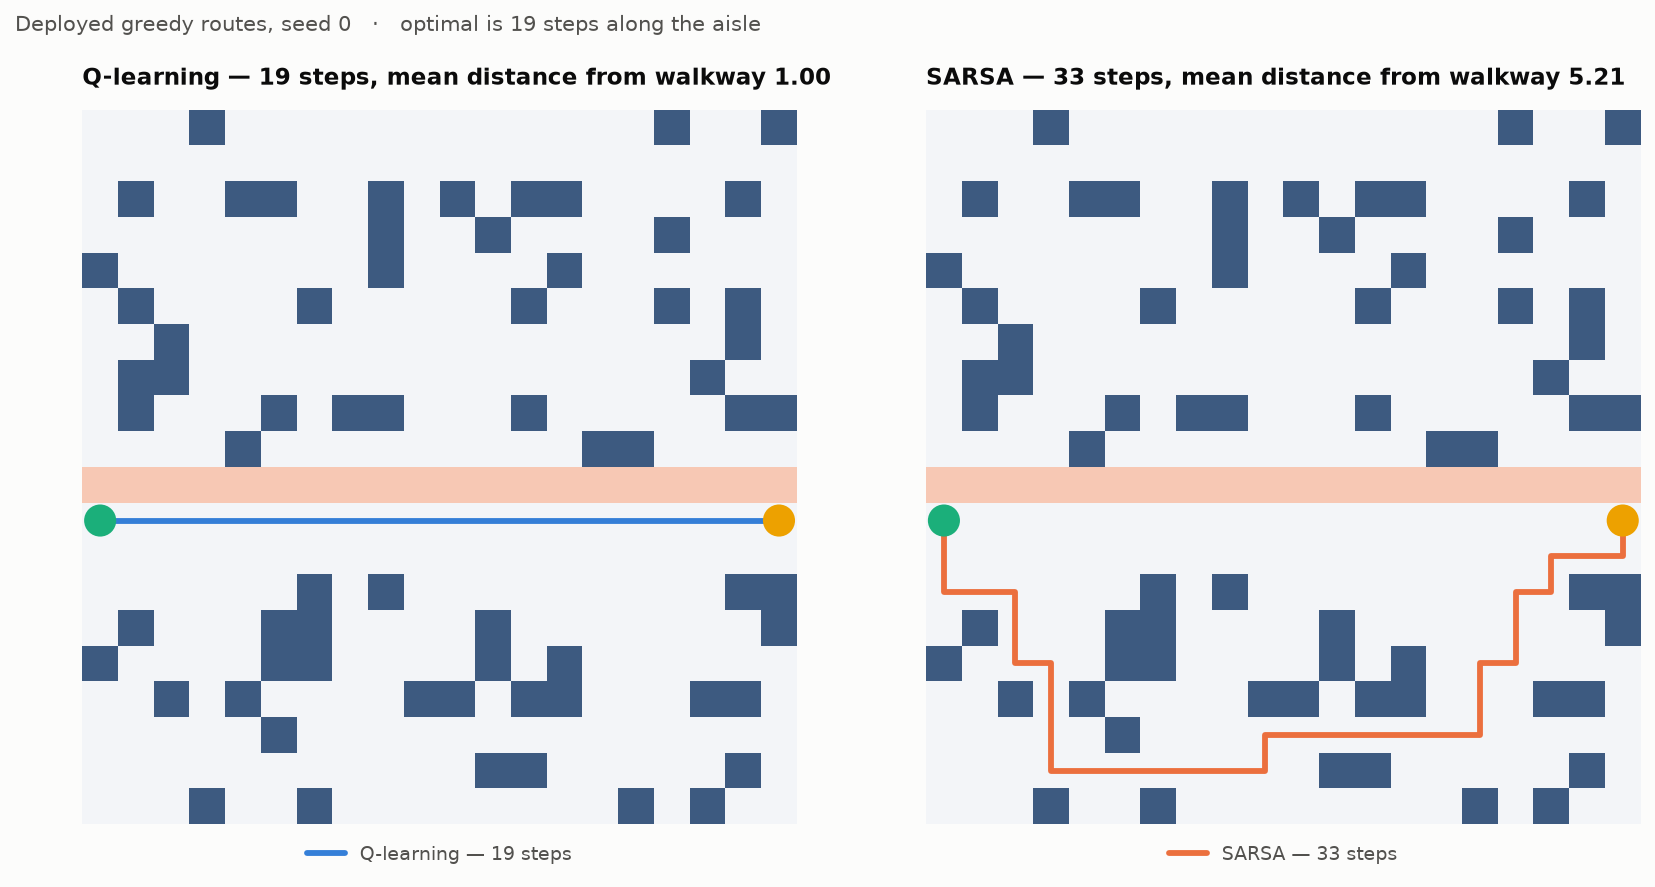
\includegraphics[width=\textwidth]{figures/fig3_learned_routes.png}
\caption[Deployed routes]{The deployed greedy routes, seed 0. Q-learning (left) runs dead straight
along the main aisle, immediately beneath the pedestrian walkway, in the optimal 19 steps. SARSA
(right) descends into the racking and takes 33 steps, averaging 5.21 cells from the walkway rather
than 1.00.}
\label{fig:routes}
\end{figure}

Figure~\ref{fig:routes} is the clearest statement of the result in the report. The two algorithms
were given identical data, identical hyperparameters and an identical experience budget, and
differed only in which policy's value they estimated. One produced a straight line along the
hazard; the other produced a detour that never approaches it.

\begin{figure}[ht]
\centering
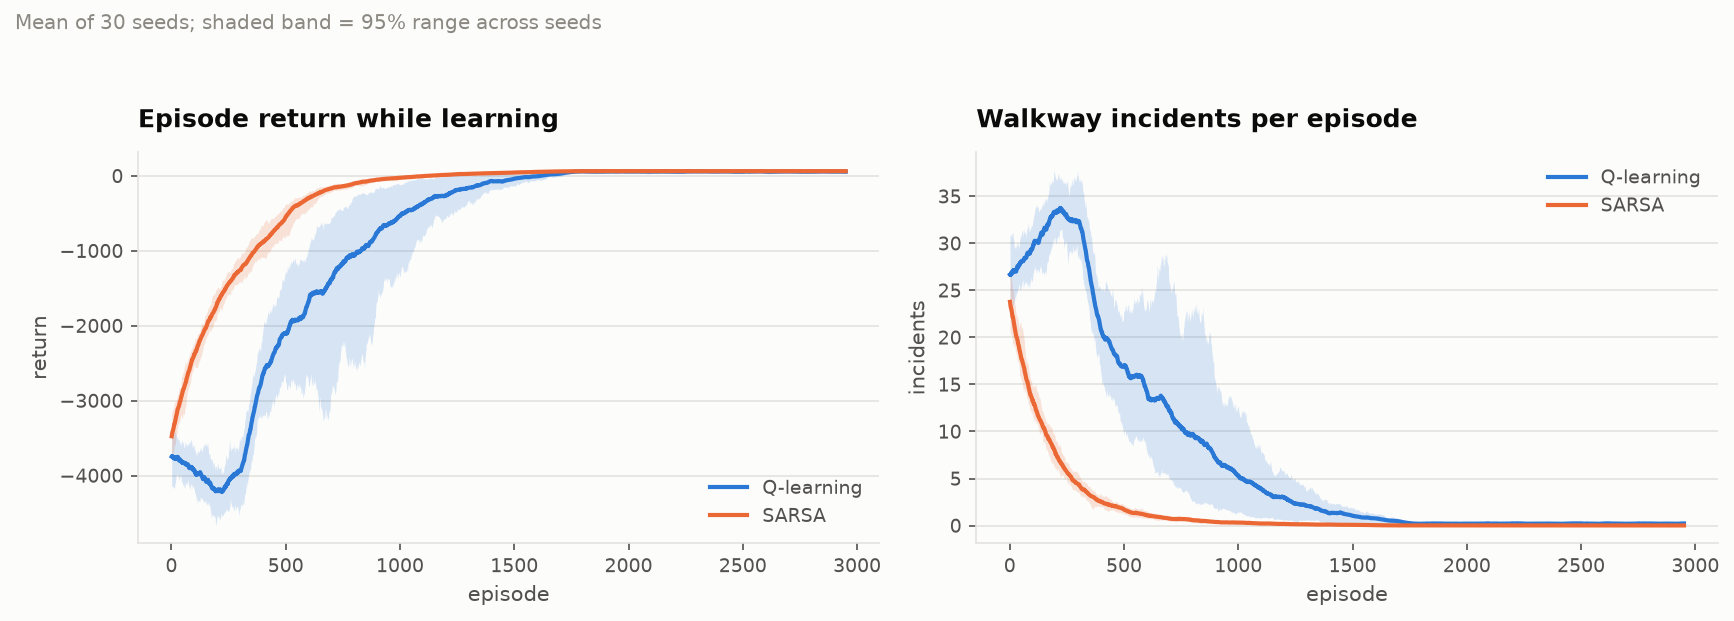
\includegraphics[width=\textwidth]{figures/fig2_learning_curves.png}
\caption[Learning curves]{Episode return and walkway incidents during training, averaged over
thirty seeds with 95\% bands. SARSA's advantage in online return is visible throughout, and is
driven by the incident rate in the right-hand panel.}
\label{fig:curves}
\end{figure}

\begin{figure}[ht]
\centering
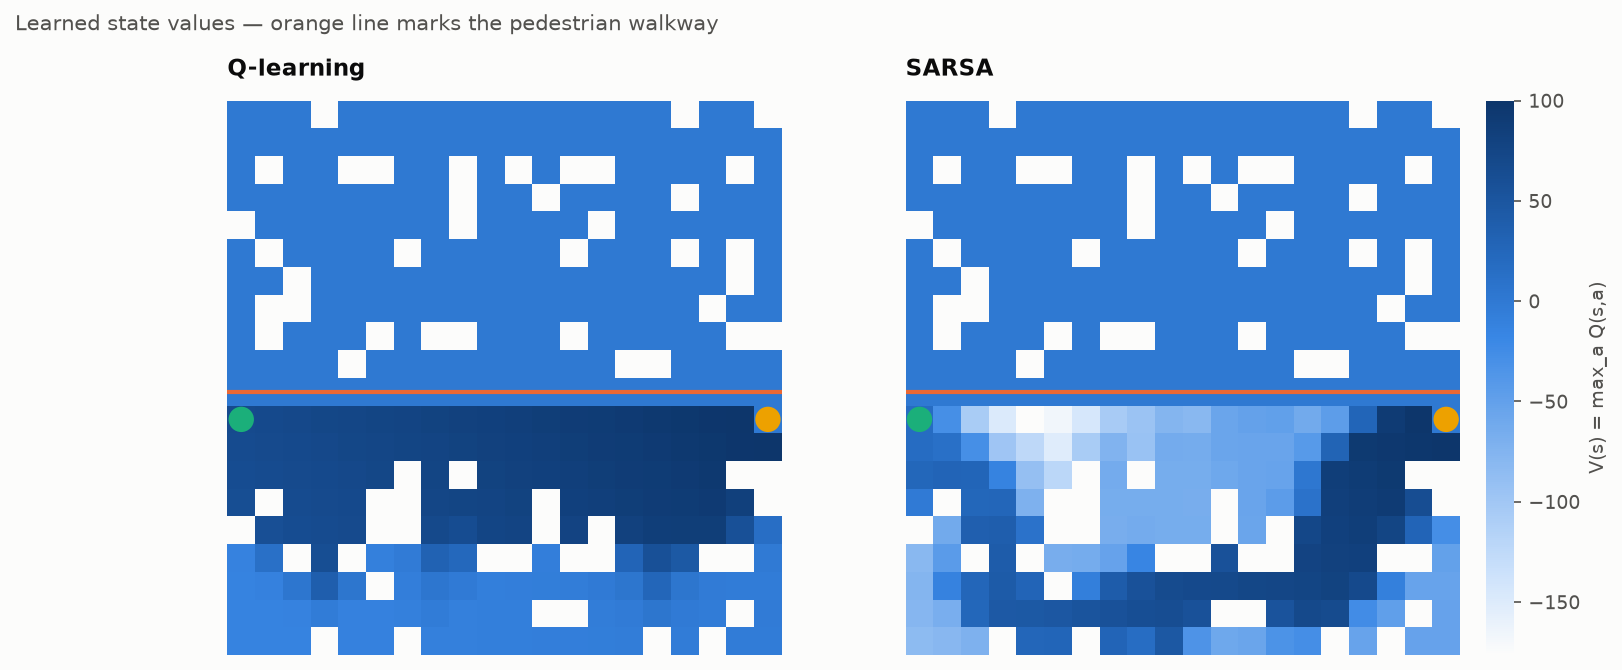
\includegraphics[width=\textwidth]{figures/fig4_value_heatmaps.png}
\caption[State values]{Learned state values $V(s) = \max_a Q(s,a)$, with the walkway marked in
orange. Q-learning assigns high value to the aisle immediately beneath the walkway; SARSA's values
are depressed in that region, which is the devaluation derived in Chapter~\ref{ch:theory} appearing
directly in the learned table.}
\label{fig:values}
\end{figure}

\begin{figure}[ht]
\centering
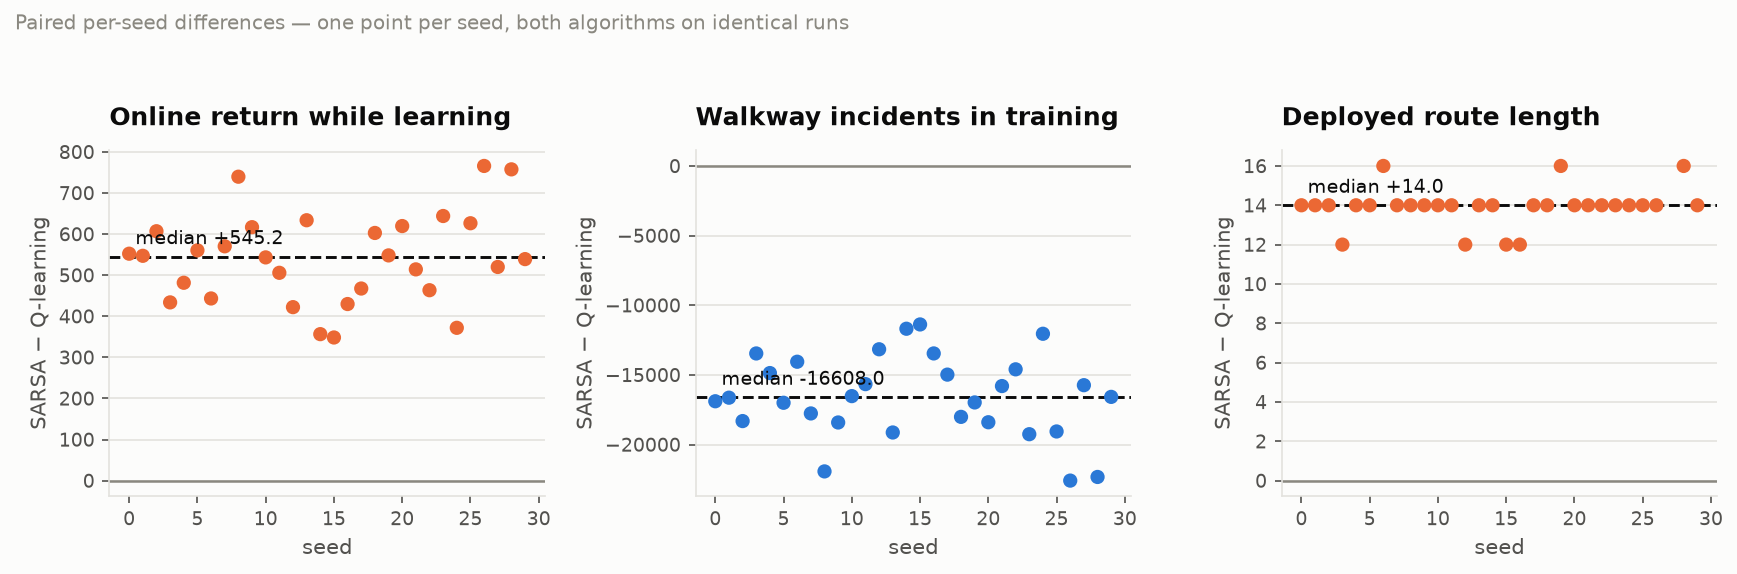
\includegraphics[width=\textwidth]{figures/fig5_paired_differences.png}
\caption[Paired differences]{Per-seed paired differences. Each point is one seed; both algorithms
were trained under identical conditions for that seed.}
\label{fig:paired}
\end{figure}

\section{External baselines}

\begin{table}[ht]
\centering
\caption[Baseline comparison]{Deployed policies against external references.}
\label{tab:baselines}
\begin{tabular}{lrrrr}
\toprule
\textbf{Policy} & \textbf{Steps} & \textbf{Success} & \textbf{Incidents} & \textbf{Return} \\
\midrule
Optimal (BFS)              & $19.00$ & $1.00$ & $0$ & $82.00$ \\
Heuristic (from the data)  & $19.00$ & $1.00$ & $0$ & $82.00$ \\
Q-learning                 & $19.40$ & $1.00$ & $0$ & $81.60$ \\
SARSA                      & $33.34$ & $0.97$ & $0$ & $-31.93$ \\
\bottomrule
\end{tabular}
\end{table}

Two observations deserve emphasis, and the second is unflattering.

First, \textbf{neither deployed policy causes any incidents}. Both algorithms learned to keep out
of the walkway; the difference between them is how much margin they leave and what that margin
cost to acquire.

Second, \textbf{the heuristic controller recovered from the dataset matches the optimum exactly},
at 19 steps with zero incidents --- equalling Q-learning and beating SARSA. This should be stated
plainly rather than buried: on this particular floor, a controller that simply moves toward the
goal is optimal, because the main aisle happens to run straight from start to goal. The heuristic
has no mechanism for handling racking that blocks its preferred direction and would fail on a floor
requiring a detour, as the generality check below indirectly shows. But on this instance it wins,
and the learned agents have not demonstrated superiority over it.

\section{Generality across floors}

\begin{table}[ht]
\centering
\caption[Generality check]{Twelve independently composed floors, each with its own racking sampled
from the dataset. ``Excess steps'' is the deployed route length minus the BFS optimum for that
floor.}
\label{tab:generality}
\begin{tabular}{lrrrr}
\toprule
\textbf{Algorithm} & \textbf{Success} & \textbf{Excess steps} & \textbf{Incidents} & \textbf{Online return} \\
\midrule
Q-learning & $1.00$ & $\mathbf{2.17}$ & $5{,}927$          & $-700.64$ \\
SARSA      & $1.00$ & $11.33$         & $\mathbf{1{,}792}$ & $\mathbf{-293.91}$ \\
\bottomrule
\end{tabular}
\end{table}

The pattern holds on every floor: Q-learning closer to optimal, SARSA with roughly a third of the
incidents. A paired Wilcoxon test on training incidents across the twelve floors gives
$p = 4.9\times10^{-4}$. The finding is not an artefact of one sampled racking arrangement.

\section{Sensitivity to the hazard penalty}

The hazard penalty is the central modelling assumption, so the experiment was repeated across a
sweep from $0$ to $-200$.

\begin{table}[ht]
\centering
\caption[Penalty sensitivity]{Sensitivity to the hazard penalty, eight seeds per cell. Q-learning's
behaviour does not change at all; SARSA's clearance rises monotonically with the penalty.}
\label{tab:sensitivity}
\begin{tabular}{lrrrr}
\toprule
\textbf{Penalty} & \multicolumn{2}{c}{\textbf{Training incidents}} & \multicolumn{2}{c}{\textbf{Distance from walkway}} \\
 & \textbf{Q-learning} & \textbf{SARSA} & \textbf{Q-learning} & \textbf{SARSA} \\
\midrule
$0$     & $401{,}268$ & $4{,}157$ & --- & $1.91$ \\
$-10$   & $6{,}522$ & $2{,}817$ & $1.74$ & $2.27$ \\
$-25$   & $6{,}522$ & $2{,}307$ & $1.74$ & $4.84$ \\
$-50$   & $6{,}522$ & $2{,}060$ & $1.74$ & $5.15$ \\
$-100$  & $6{,}522$ & $1{,}947$ & $1.74$ & $5.25$ \\
$-200$  & $6{,}522$ & $1{,}844$ & $1.74$ & $5.39$ \\
\bottomrule
\end{tabular}
\end{table}

\begin{figure}[ht]
\centering
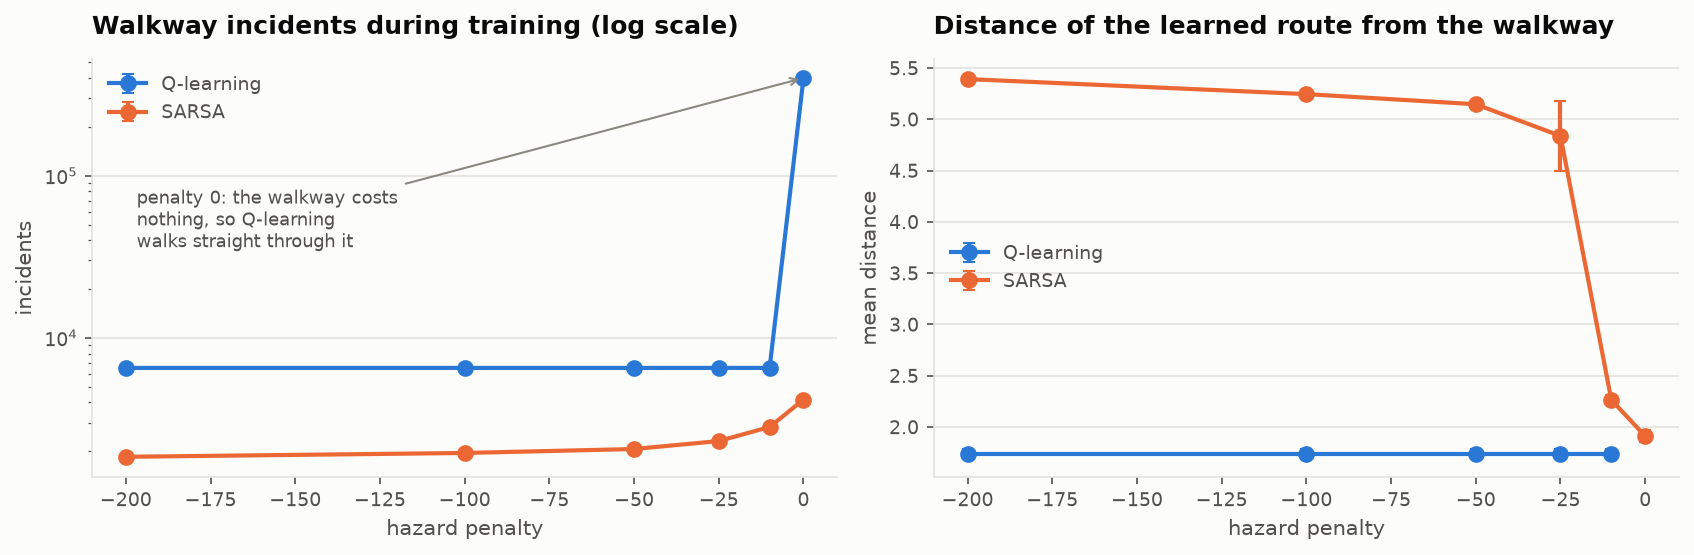
\includegraphics[width=\textwidth]{figures/fig6_penalty_sensitivity.png}
\caption[Penalty sensitivity]{Sensitivity to the hazard penalty. Incidents are plotted on a log
scale because the zero-penalty case is two orders of magnitude above the rest.}
\label{fig:sensitivity}
\end{figure}

This table contains the single most informative result in the report, and it is not the headline
one.

\keypoint{Q-learning's behaviour is completely invariant to the hazard penalty.} Its incident count
is identical --- $6{,}522$ --- at every penalty from $-10$ to $-200$, and its distance from the
walkway is $1.74$ throughout. A twenty-fold increase in the cost of an incident changes its
behaviour by nothing at all.

This is exactly what Chapter~\ref{ch:theory} predicts. Q-learning backs up through
$\max_a Q(s,a)$, which selects the safe action, so the penalty attaches to
$Q(s, a_{\text{bad}})$ but never propagates into $V(s)$. The states beside the walkway are
therefore never devalued however large the penalty becomes. The mechanism is not inferred from the
outcome here --- it is directly visible in the measurements.

\keypoint{SARSA responds monotonically.} Its clearance rises from $1.91$ at zero penalty to $5.39$
at $-200$, and its incidents fall correspondingly. The on-policy backup carries an
$\varepsilon/|\mathcal{A}|$-weighted share of the penalty into the state value, so a larger
penalty produces a wider berth.

\keypoint{At zero penalty the effect disappears, and Q-learning degenerates.} With no cost,
entering the walkway is a free teleport back to the start, and Q-learning's greedy policy cycles
through it indefinitely --- 401{,}268 incidents, and it fails to reach the goal at all. This is the
degenerate end of the sweep rather than a tuning failure, and it is reported because it
demonstrates that the hazard penalty is not a free parameter that can be set to taste.
